%\documentclass[a4paper,twoside,11pt,open=any]{scrbook}
%damit die erste Seite einer Übung immer links gelocht ist:
\documentclass[a4paper,twoside,11pt,open=any]{scrbook}

\usepackage{fancyhdr}

\usepackage[utf8]{inputenc}							%für deutsche Sonderzeichen
\usepackage[ngerman]{babel}									%für deutsches Datum
\usepackage[babel,german=quotes]{csquotes}	%deutsche Anführungszeichen
\usepackage[T1]{fontenc}										%für Umlaute und Akzente
\usepackage{graphicx}												%für Grafiken
\usepackage{newcent}												%für Skalierbarkeit der Schrift
\usepackage{amsmath}												%Verbesserung der Formeln
\usepackage{cancel}													%kürzen in Formeln
\usepackage{ulem}
\usepackage{enumitem} 											%Aufzählungen

\usepackage{geometry}
\geometry{a4paper,left=25mm,right=15mm, top=10mm, bottom=25mm}

\geometry{left=25mm, right=10mm}
\geometry{top=30mm,bottom=30mm}
\geometry{headheight=20mm}
\geometry{headsep=5mm}
\geometry{footskip=10mm} 

\usepackage{xcolor}
\definecolor{white} {rgb}{255, 255, 255}
\definecolor{red} {rgb}{255, 0, 0}
\usepackage[pdfstartview=FitBH, breaklinks = true, citebordercolor = white, linkbordercolor = white, urlbordercolor  = white]{hyperref}
\hypersetup
{
	pdftitle = {Softwareprojekt: Kundenprojekt II: Webtechnologien, Gruppendokumentation},
	pdfsubject = {Tom Bullmann},
	pdfkeywords = {LaTeX, swp, Softwareprojekt},
	pdfauthor = {Tom Bullmann},
}

\renewcommand \thechapter {\Roman{chapter}}
\renewcommand \thesection {\arabic{section}}
\usepackage{tocloft} 
\setlength{\cftsecnumwidth}{5.5em} % damit der lange String "Aufgabe 1" passt

\renewcommand*\chapterheadstartvskip{\vspace*{0mm}}


\usepackage{listings}
\lstset{language=C,numbers=left,xleftmargin=10mm
,commentstyle=\small\selectfont,basicstyle=\ttfamily\small\selectfont
}

\usepackage{tabularx}

%\lstset{}

	\fancypagestyle{plain}{
		\fancyhf{}
		\fancyhead[OL,ER]{SS 12 \\ \today}
		\fancyhead[C]{\textbf{Softwareprojekt: Kundenprojekt II - Webtechnologien \ifnum0<\arabic{chapter}  -
\arabic{chapter}.\hspace{0.5em}Woche \fi} \\ Dozentin: Prof. Dr. M\"uller-Birn}
		\fancyhead[OR,EL]{Team 1}
		\renewcommand{\headrulewidth}{0.4pt} %obere Trennlinie
		\fancyfoot[OR,EL]{\smallskip \thepage} %Seitennummer
		\fancyfoot[C]{\tiny{Freie Universit\"at Berlin\\ Fachbereich Mathematik und Informatik\\ Institut f\"ur Informatik}}
		\renewcommand{\footrulewidth}{0.4pt} %untere Trennlinie
	}

\begin{document}
  \pagestyle{plain}
  \begin{titlepage}
  \begin{center}
    \Large
    \textsc
    {
    	\\
    	\vspace{2cm}
    	Softwareprojekt: Kundenprojekt II \\ Webtechnologien
    }\\
  	\vspace{5cm}
  	\textsc
  	{
  		Gruppendokumentation\\[0.5\baselineskip]
  		von\\[0.5\baselineskip]
  		Team 1\\
		\begin{tiny}
			Tom Bullmann\hspace{1cm}Andreas N\"u\ss{}lein\hspace{1cm}Sebastian Schulz\hspace{1cm}Mareike Ziese\\
		\end{tiny}
  	}
  	\vspace{5cm}
    \textsc{\today}\\
    \vspace{1cm}
    \textsc
    {
    	Dozentin:\\
    	Prof. Dr. M\"uller-Birn
    }\\
  	\vspace{1cm}
  	\textsc{
  		Freie Universit\"at Berlin\\
  		Fachbereich Mathematik und Informatik\\
  		Institut f\"ur Informatik
  	}\\
  \end{center}
\end{titlepage}
  \tableofcontents
  \clearpage
  \chapter{Introduction}\label{wo1}

The sole purpose of this document is to describe the complete process of the project, which was done in the cooperation of the
Carmeq GmbH and the Free University of Berlin, with the topic of intermodal passenger transportation.

At the beginning of this course there were 18 students enrolled for this course. They have been divided into 4 teams, which
worked separately from the beginning. 
  \chapter{Emphasise}\label{wo2}

  \chapter{Define}\label{wo3}


  \chapter{Ideate}\label{wo4}


  \chapter{Paper-Prototype}\label{wo5}


  \chapter{Prototype}\label{wo6}

\section{Database}\label{wo6_1}

\begin{center}
	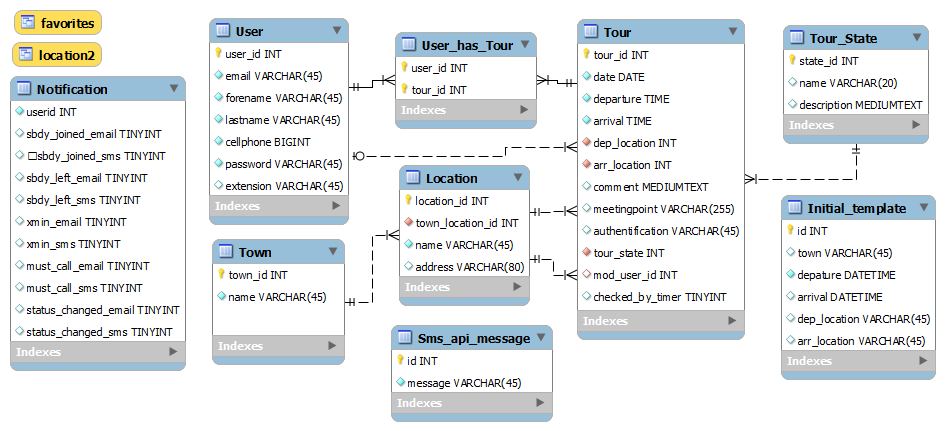
\includegraphics[width=17cm]{img/Datenbank_Model}
\end{center}

\section{Architecture}\label{wo6_2}

\begin{center}
	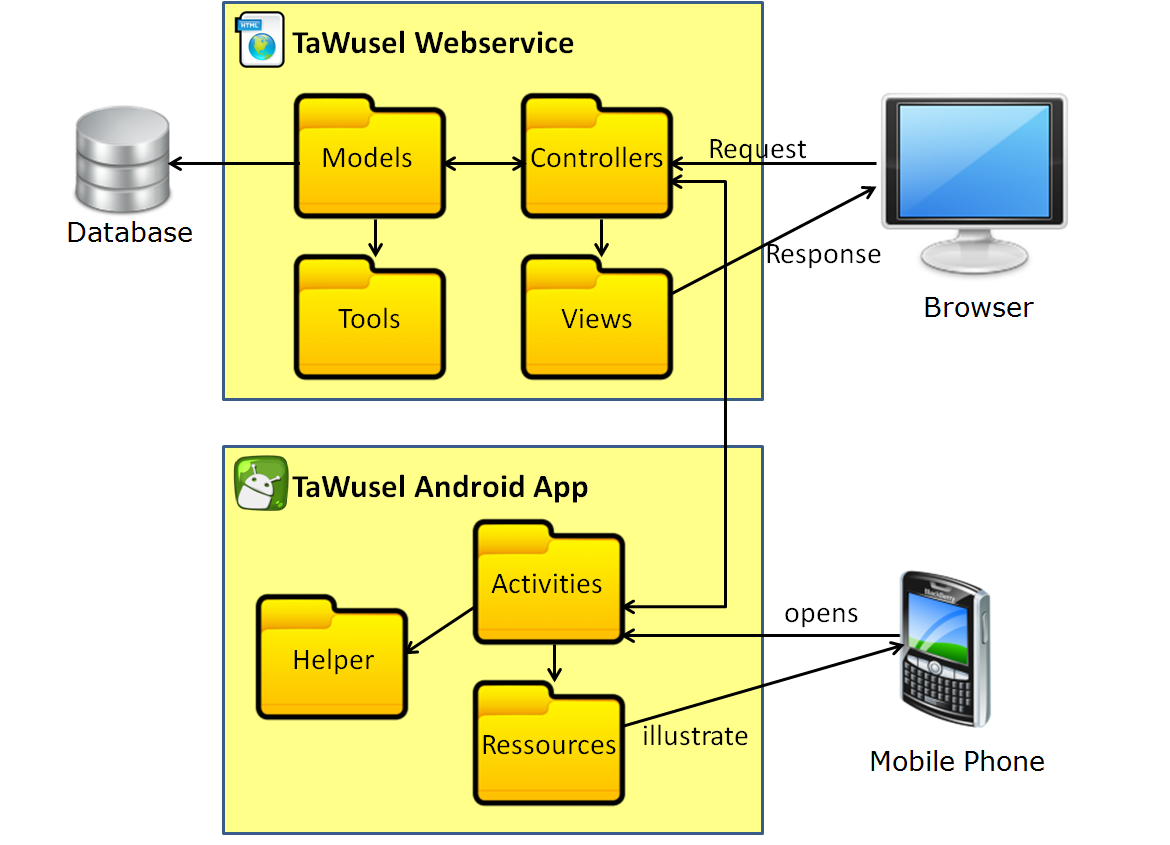
\includegraphics[width=17cm]{img/Architekturdiagramm}
\end{center}


\section{Installation guide - web-application}\label{wo6_3}

\textbf{1.} Grab play from http://www.playframework.org/ and install it.

\textbf{1.1.} Basically it is: unzip, add to \$PATH and run it. Or follow these instructions:
http://www.playframework.org/documentation/2.0.2/Installing\\
\textbf{2.} Set up a mysql-database for this project, e.g.:

CREATE DATABASE tawusel; GRANT ALL ON tawusel.* TO tawusel@localhost IDENTIFIED BY 'pass'; (if you want to use other credentials,
change file conf/application.conf accordingly)\\
\textbf{3.} In the project's root folder (i.e. here) run play run\\

Point web browser to http://localhost:9000/

\section{Installation guide - Android-application}\label{wo6_4}

\textbf{1.} Make sure you locate the tawusel.properties into the assets folder. Here you have to replace the json server
property ("http://10.0.2.2:9000/") by the address of the server your tawusel service is running on.\\
\textbf{2.} Generate your tawusel.apk.\\
\textbf{3.} Install the apk on your mobile phone.\\
(remark: the current version works stable on android 2.3.3 but its working on higher versions is not guaranteed)

\end{document}